\appendix
\chapter{Pseudocode Listings}
\begin{algorithm}[caption={Kinship Term Reduction}, label={algo:red}]
    input: kinship term $t$.
    note: $\omega$ is a dictionary of kinship terms.
    note: Functions "leftPart(t, u)" and "rightPart(t, u)" return the sub-term of $t$
    note: from the left of sub-term $u$ or from the right respectively.
    note: Function "subterm(t, i, j)" returns the
    note: sub-term of the kinship term $t$ between indices $i$ and $j$.
    output: reduced kin term.
    function shorten(t)
    begin
        maxShortenableSubterm $\gets$ empty
        currentSubterm $\gets$ empty
        for i $\gets$ 0 to length(t) do
        begin
            for j $gets$ length(t) - i to 0 do
            begin
                currentSubterm $\gets$ subterm(t, i, j)
                if length(currentSubterm) $>$ length(maxShortenableSubterm)
                    and $\omega$(currentSubterm) is not empty
                then
                    maxShortenableSubterm = currentSubterm
            end
        end
        return shorten(leftPart(t, maxShortenableSubterm))
               $\cdot$ $\omega(maxShortenableSubterm)$
               $\cdot$ shorten(rightPart(t, maxShortenableSubterm))
    end
\end{algorithm}

\chapter{Figures}
\begin{figure}[h!]
    \centering
    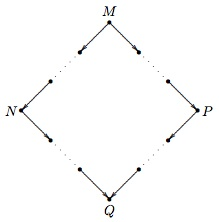
\includegraphics{figs/confluence.jpg}
    \caption{Confluence in a term rewriting system.}
    \label{fig:conf}
\end{figure}
